% $Header: /home/vedranm/bitbucket/beamer/solutions/conference-talks/conference-ornate-20min.en.tex,v 90e850259b8b 2007/01/28 20:48:30 tantau $

\documentclass[compress]{beamer}

% This file is a solution template for:

% - Talk at a conference/colloquium.
% - Talk length is about 20min.
% - Style is ornate.



% Copyright 2004 by Till Tantau <tantau@users.sourceforge.net>.
%
% In principle, this file can be redistributed and/or modified under
% the terms of the GNU Public License, version 2.
%
% However, this file is supposed to be a template to be modified
% for your own needs. For this reason, if you use this file as a
% template and not specifically distribute it as part of a another
% package/program, I grant the extra permission to freely copy and
% modify this file as you see fit and even to delete this copyright
% notice. 


\mode<presentation>
{
  \usetheme{Warsaw}
  % or ...

  \setbeamercovered{transparent}
  % or whatever (possibly just delete it)
}


\usepackage[english]{babel}
% or whatever

\usepackage[latin1]{inputenc}
% or whatever

\usepackage{times}
\usepackage[T1]{fontenc}
% Or whatever. Note that the encoding and the font should match. If T1
% does not look nice, try deleting the line with the fontenc.
\usepackage{graphicx}

\title{Cleaning point cloud vegetation}

\author{Rickert Mulder}
% - Give the names in the same order as the appear in the paper.
% - Use the \inst{?} command only if the authors have different
%   affiliation.

\institute[U of X]
{
  Department of Computer Science\\
  University of Cape Town
}

\date[CFP 2003] % (optional, should be abbreviation of conference name)
{Masters Proposal}
% - Either use conference name or its abbreviation.
% - Not really informative to the audience, more for people (including
%   yourself) who are reading the slides online

\subject{Computer Science}
% This is only inserted into the PDF information catalog. Can be left
% out. 



% If you have a file called "university-logo-filename.xxx", where xxx
% is a graphic format that can be processed by latex or pdflatex,
% resp., then you can add a logo as follows:

\pgfdeclareimage[height=1.0cm]{university-logo}{pics/UCT}
\logo{\pgfuseimage{university-logo}}



% Delete this, if you do not want the table of contents to pop up at
% the beginning of each subsection:
%\AtBeginSubsection[]
%{
%  \begin{frame}<beamer>{Outline}
%    \tableofcontents[currentsection,currentsubsection]
%  \end{frame}
%}


% If you wish to uncover everything in a step-wise fashion, uncomment
% the following command: 

%\beamerdefaultoverlayspecification{<+->}


\begin{document}

\begin{frame}
  \titlepage
\end{frame}

\begin{frame}{Outline}
  \tableofcontents
  % You might wish to add the option [pausesections]
\end{frame}


% Structuring a talk is a difficult task and the following structure
% may not be suitable. Here are some rules that apply for this
% solution: 

% - Exactly two or three sections (other than the summary).
% - At *most* three subsections per section.
% - Talk about 30s to 2min per frame. So there should be between about
%   15 and 30 frames, all told.

% - A conference audience is likely to know very little of what you
%   are going to talk about. So *simplify*!
% - In a 20min talk, getting the main ideas across is hard
%   enough. Leave out details, even if it means being less precise than
%   you think necessary.
% - If you omit details that are vital to the proof/implementation,
%   just say so once. Everybody will be happy with that.

\section{Introduction}

\subsection*{Introduction}
\begin{frame}{Aim}

\begin{columns}[T]
\begin{column}{1.0\textwidth}

\begin{itemize}
\item  Improve the speed at which vegetation can be removed from point clouds without sacrificing accuracy
% what is a lazer scan?
\end{itemize}

\centering
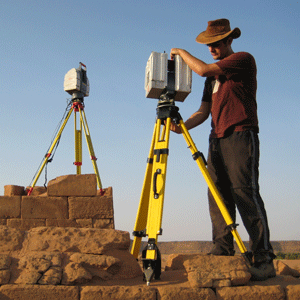
\includegraphics[height=0.5\textheight]{pics/zamani4}
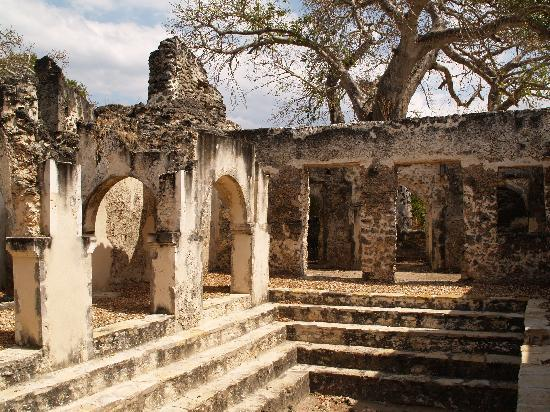
\includegraphics[height=0.5\textheight]{pics/zamani3}

\end{column}
\begin{column}{0.0\textwidth}

\end{column}
\end{columns}


\end{frame}

\section{Motivation}

\subsection{Background}

\begin{frame}{The Zamani Project}
  % - A title should summarize the slide in an understandable fashion
  %   for anyone how does not follow everything on the slide itself.

  
\includegraphics[width=0.70\textwidth]{pics/Zamani_logo}

  \begin{itemize}
  \item Cultural heritage preservation
  \item Document heritage sites in 3D 
  \end{itemize}
\end{frame}

\begin{frame}{Data capture}
	% There are many ways in which this can be done
    % Structured light, structure from motion, traingulation

  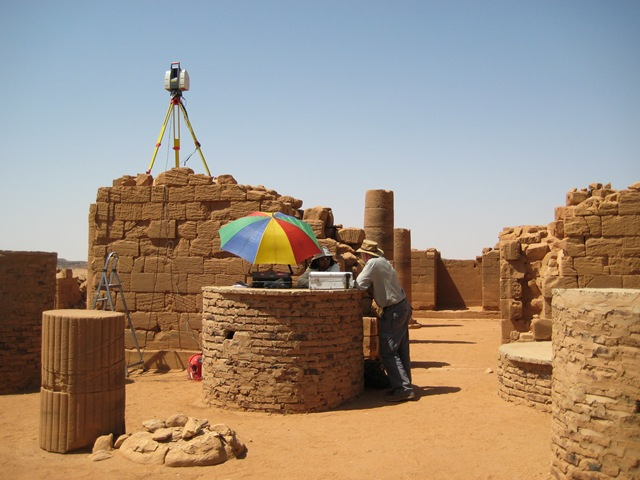
\includegraphics[width=0.60\textwidth]{pics/scanning.jpg}
    \begin{itemize}
  \item
    Laser range scanning
  \item
    Site photography
  \end{itemize}
\end{frame}

\begin{frame}{Processing Pipeline}
  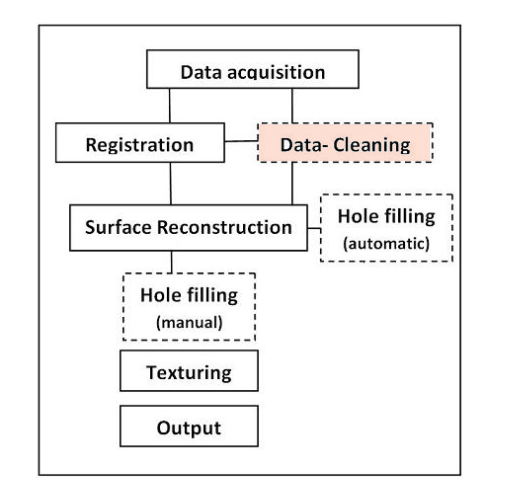
\includegraphics[width=0.50\textwidth]{pics/pipeline.png}
  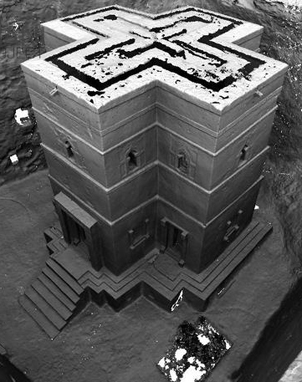
\includegraphics[width=0.38\textwidth]{pics/zamani2.jpg}
\end{frame}

\begin{frame}{Cleaning}
\centering
  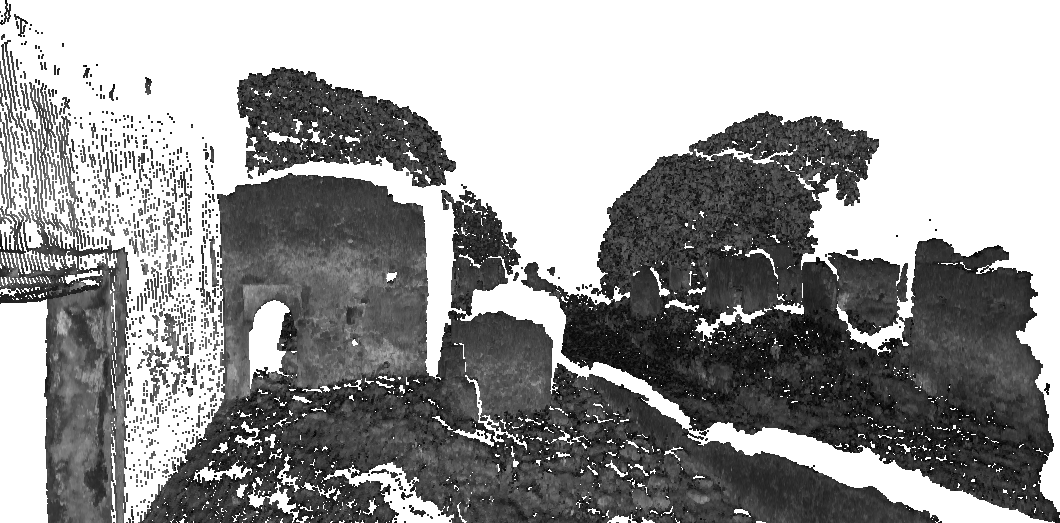
\includegraphics[width=1\textwidth]{pics/dirty}
  \begin{itemize}
  \item
  Cleaning is the removal of unwanted objects or noise
  \item
  Involves classification and segmentation
  \end{itemize}
\end{frame}

\begin{frame}{Problem}
  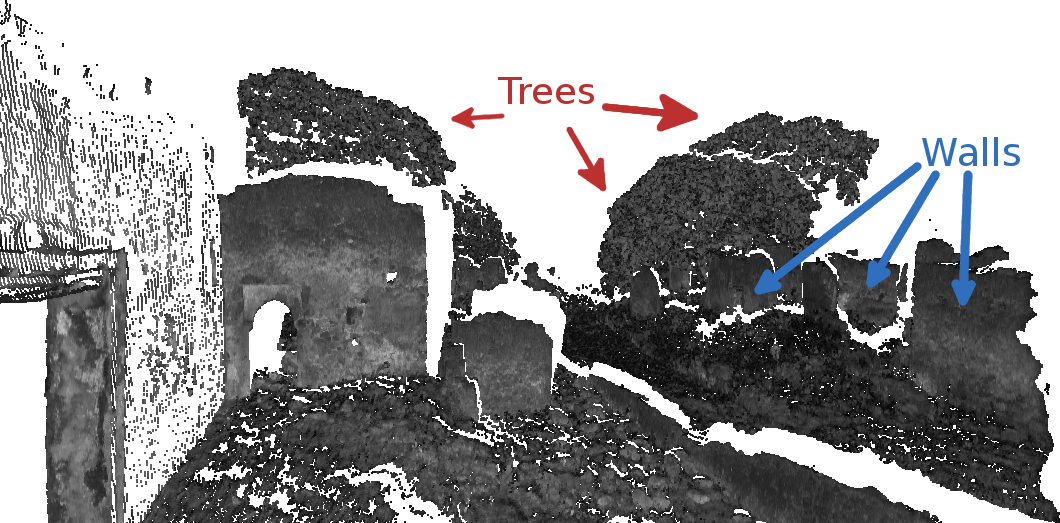
\includegraphics[width=1\textwidth]{pics/dirty2}
  \begin{itemize}
  \item
  500 - 1000 scans per expedition
  \item
  30 min to 2 hours per scan
  \item
  Vegetation is the hardest type of noise to remove
  \item
  Focus on accuracy
  % duplication of work
  % more memory requirements
  % size of data input should be noted
  % not only Zamani but also CyArk
  \end{itemize}
\end{frame}

\subsection{Related Work}

\begin{frame}{Existing software}
% Existing software is often sluggish also
% response times plays a big role

\centering



\includegraphics[height=0.10\textheight]{pics/cyclone.jpg}

\includegraphics[height=0.10\textheight]{pics/pointools.jpg}

\includegraphics[height=0.10\textheight]{pics/meshlab.png}
%includegraphics[height=0.10\textheight]{pics/vrmesh.png}

\includegraphics[height=0.10\textheight]{pics/3dreshaper.jpg}
\vskip0pt plus.5fill
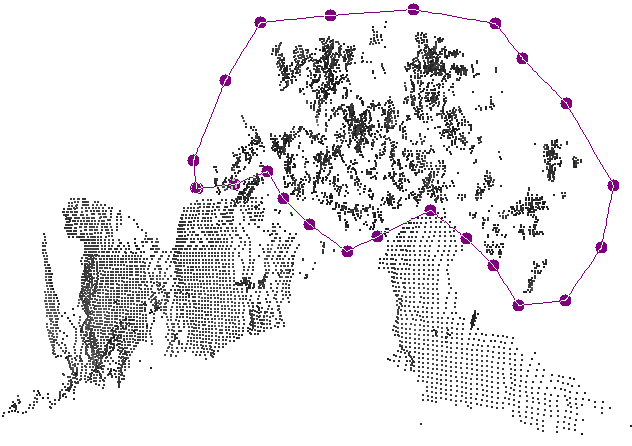
\includegraphics[height=0.40\textheight]{pics/lasso.png}
%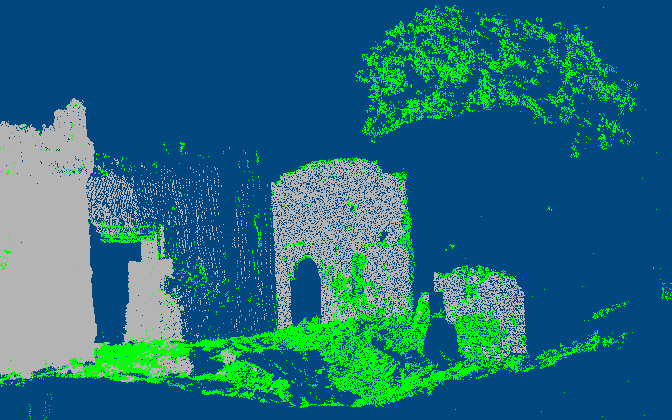
\includegraphics[width=0.50\textwidth]{pics/vrmesh-veg.png}
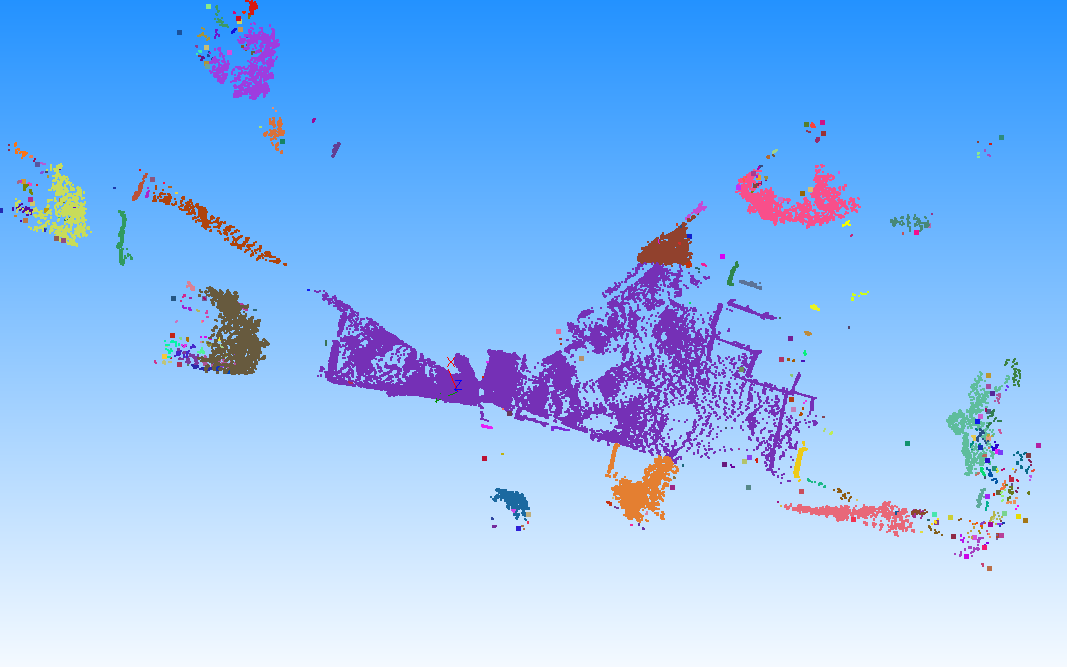
\includegraphics[height=0.40\textheight]{pics/clustering.png}
\\

\begin{itemize}
\item
  Various levels of user intervention
\end{itemize}
%Existing tools vary in terms of
%\begin{itemize}
%\item automation
%\item accuracy
%\end{itemize}

%\begin{itemize}
%\item Leica Cyclone (used by Zamani)
%\item Pointools Edit (used by CyArk)
%\item Meshlab
%\item VR Mesh Studio
%\item Terrascan
%\item 3D Reshaper
%\item Carlson PointCloud
%\end{itemize}

\end{frame}

\begin{frame}{Vegetation classification}

\centering
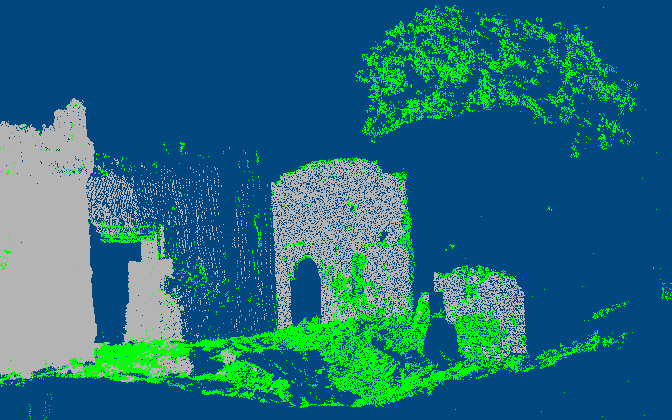
\includegraphics[width=0.9\textwidth]{pics/vrmesh-veg.png}
\begin{itemize}
\item Leaves much to be desired
\end{itemize}

\end{frame}

\section{Proposal}

\subsection{Aim}

\begin{frame}{Goal}
\begin{itemize}

\item
Create semi-automated tools to accurately segment vegetation in point clouds in a way that is fast and accurate.

\begin{itemize}
\item Allow user to make crude segmentation
\item Refine segmentation computationally
\end{itemize}

\end{itemize}

\end{frame}

%\begin{frame}{Research Questions}
%
%\begin{itemize}
%\item To what extent can augmented methods speed up the segmentation of vegetation?
%\item What degree of accuracy can be obtained?
%\end{itemize}
%
%\end{frame}

\begin{frame}{Point cloud segmentation \& classification}

\begin{columns}[T]
\begin{column}{0.5\textwidth}

\begin{itemize}
\item Point features
\item Classify points:
\begin{itemize}
\item Heuristics
\item Classifiers
\end{itemize}
\end{itemize}

\end{column}

\begin{column}{0.5\textwidth}


\includegraphics[width=1\textwidth]{pics/features.png}

\end{column}
\end{columns}
\end{frame}

\begin{frame}{System}

\begin{columns}[T]
\begin{column}{0.7\textwidth}

\begin{itemize}

\item Use Point Cloud Library (PCL)
\item Focus on responsiveness

\begin{itemize}
\item Point feature calculations can be costly
\item Push load to GPU
\end{itemize}

\item Built in collaboration with Zamani
\item Iterative Prototyping

\end{itemize}


\end{column}
\begin{column}{0.3\textwidth}


\includegraphics[height=0.5\textheight]{pics/pcl_vert_large_pos.png}

\end{column}
\end{columns}

\end{frame}

\subsection{Evaluation}

\begin{frame}{Evaluation}
\begin{columns}[T]
\begin{column}{0.6\textwidth}
	\begin{itemize}
		\item Expert opinion
		\item User study to measure time and accuracy
		\item Compare results to existing system 
	\end{itemize}
	
\end{column}
\begin{column}{0.4\textwidth}
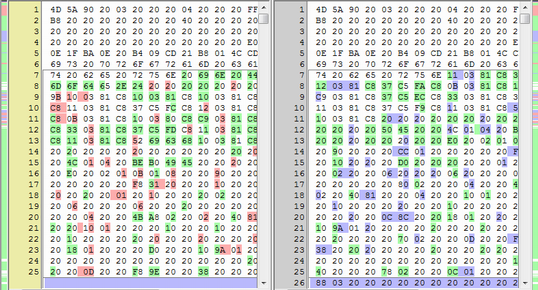
\includegraphics[width=1\textwidth]{pics/diff.png}
\end{column}
\end{columns}
\end{frame}

\begin{frame}{System thus far}
\begin{columns}[T]
\begin{column}{1\textwidth}
	\begin{itemize}
		\item Pluggable point cloud cleaning framework
		\item Lasso tool, flood fill, brush tool
	\end{itemize}
	
\centering
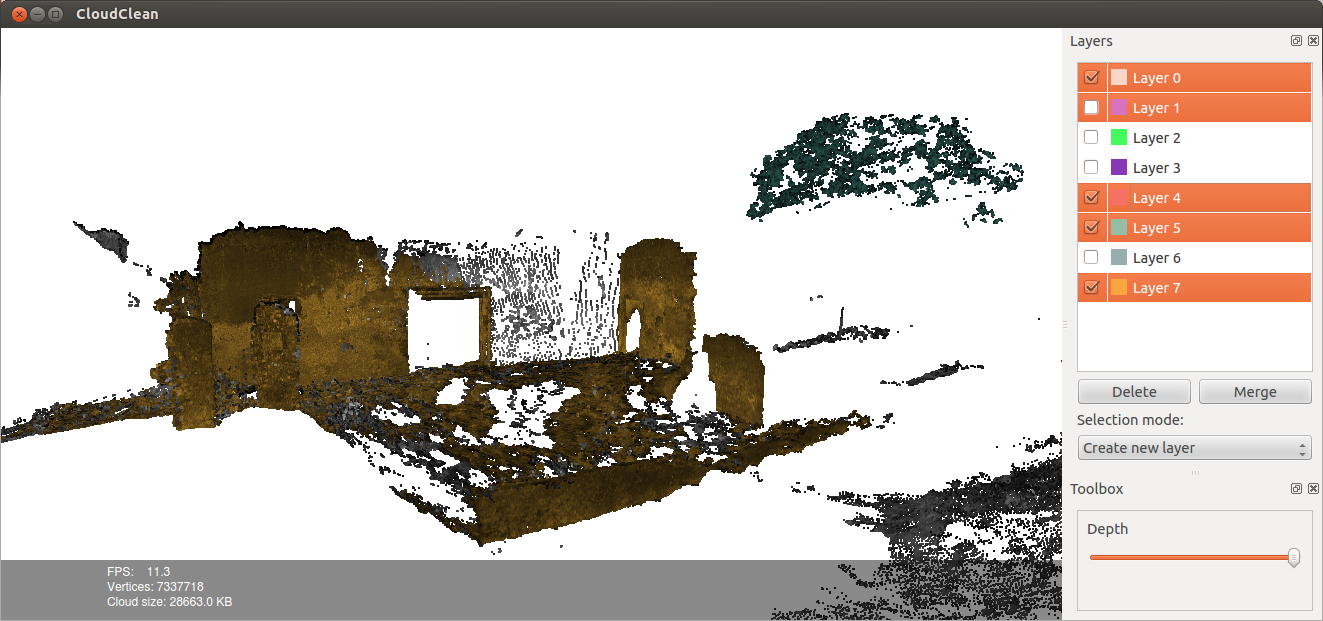
\includegraphics[height=0.45\textheight]{pics/myapp3.png}
\end{column}
\begin{column}{0.0\textwidth}

\end{column}
\end{columns}
\end{frame}


% All of the following is optional and typically not needed. 
\appendix
\section<presentation>*{\appendixname}
\subsection<presentation>*{For Further Reading}

\begin{frame}{Questions?}

\centering
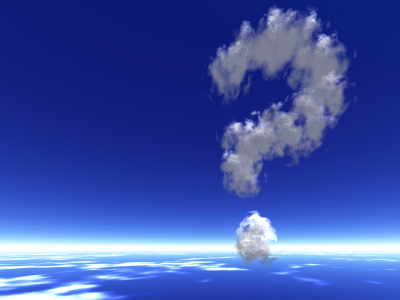
\includegraphics[height=0.45\textheight]{pics/questions}

\end{frame}

\subsection{Project plan}
\begin{frame}{Timeline}
\begin{table}[h]
\begin{tabular}{llr}
Research Proposal & 13 June 2012\\
Point Cloud Cleaning Framework & 30 June 2012\\
Clean Isolated Vegetation & 7 September 2012\\
Clean Co-occurring Vegetation & 15 November 2013\\
Background Chapter & 22 November 2012\\
System Design Chapter & 7 January 2013\\
GPGPU port & 15 January 2012\\
Implementation Chapter & 22 February 2013\\
User testing & 28 February 2012\\ % will they have interns yet?
Evaluation Chapter & 7 March 2013\\
Thesis Draft & 7 April 2013\\
Conference Paper & 7 May 2013\\
Final Draft & 7 July 2013\\
\end{tabular}
\end{table}
\end{frame}

\begin{frame}{Risk}
\begin{columns}[T]
\begin{column}{0.5\textwidth}
	\begin{itemize}
	    \item Limited number of test users
		\item Reliance on the Zamani project
		\item Difficulty under/overestimated
	\end{itemize}
\end{column}
\begin{column}{0.5\textwidth}
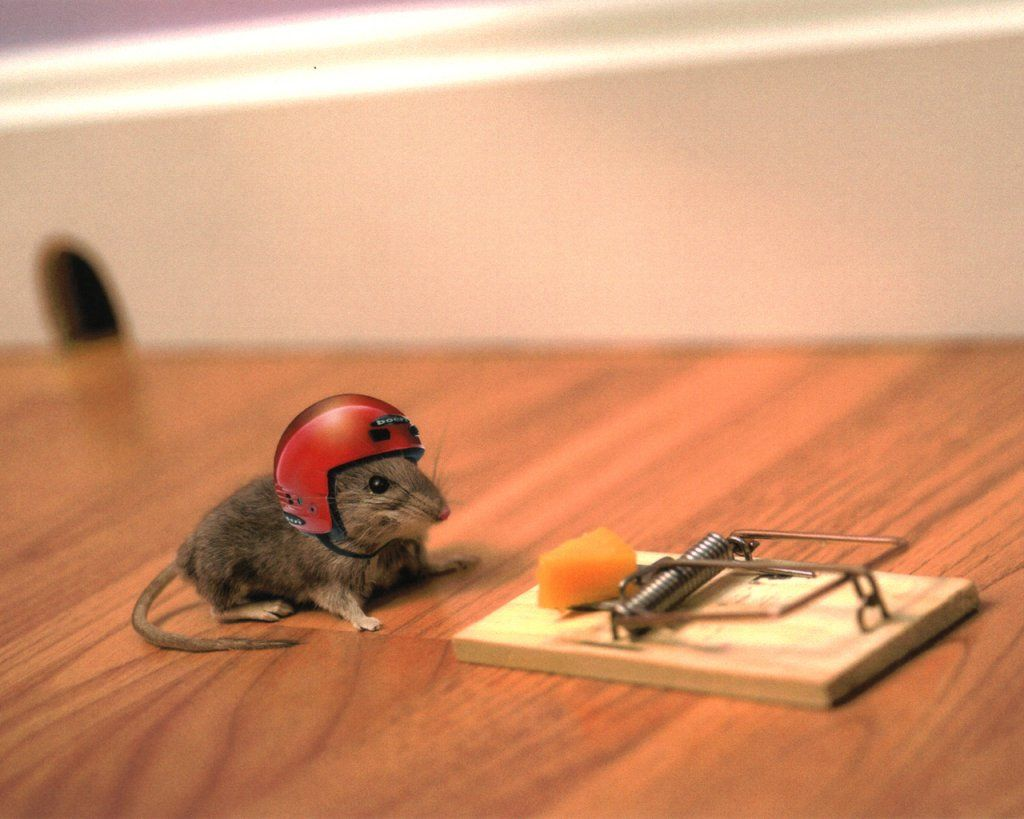
\includegraphics[width=0.7\textwidth]{pics/risk2}
\end{column}
\end{columns}
\end{frame}


\begin{frame}{Related work}

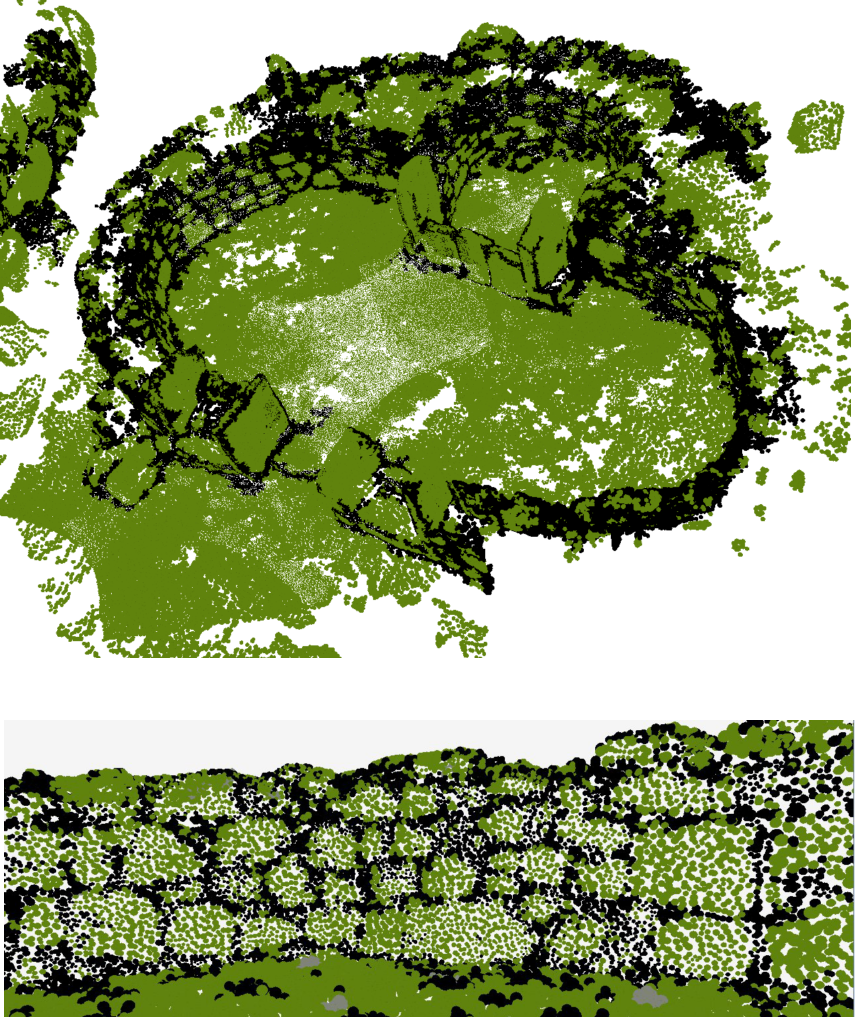
\includegraphics[width=0.4\textwidth]{pics/spina2.png}
% spina cultural heritage
% 600k points
% many unclassified
% principal components
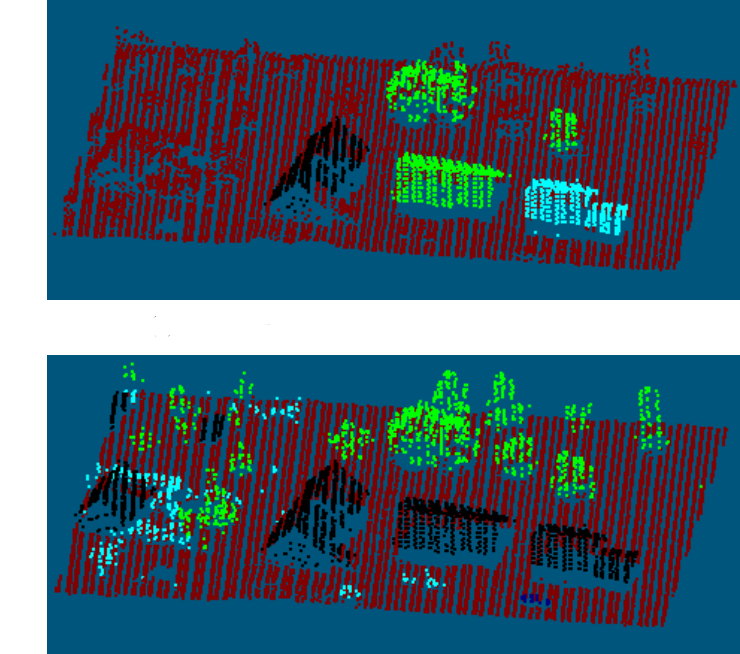
\includegraphics[width=0.5\textwidth]{pics/shapovalov.png}
% uses probalitic models
% Associative makov networks
% Conditional random fields
% airial scans less dense

\end{frame}

%\begin{frame}[allowframebreaks]
%  \frametitle<presentation>{For Further Reading}
%    
%  \begin{thebibliography}{10}
%    
%  \beamertemplatebookbibitems
%  % Start with overview books.
%
%  \bibitem{Author1990}
%    A.~Author.
%    \newblock {\em Handbook of Everything}.
%    \newblock Some Press, 1990.
% 
%    
%  \beamertemplatearticlebibitems
%  % Followed by interesting articles. Keep the list short. 
%
%  \bibitem{Someone2000}
%    S.~Someone.
%    \newblock On this and that.
%    \newblock {\em Journal of This and That}, 2(1):50--100,
%    2000.
%  \end{thebibliography}
%\end{frame}

\end{document}
